\documentclass[a4paper]{article}

%% Language and font encodings
\usepackage[english]{babel}
\usepackage[utf8]{inputenc}
\usepackage[T1]{fontenc}

%% Page size and margins
\usepackage[a4paper,top=2cm,bottom=2cm,left=2.5cm,right=2.5cm,marginparwidth=1.75cm]{geometry}

%% Core packages
\usepackage{amsmath}
\usepackage{graphicx}
\usepackage{tabularx}
\usepackage{booktabs}
\usepackage{float}
\usepackage{subcaption}
\usepackage{microtype}
\usepackage{xcolor}
\definecolor{tcdBlue}{RGB}{5, 105, 185}
\usepackage{tikz}
\usetikzlibrary{shapes.geometric, arrows.meta, positioning, fit, backgrounds}

%% Hyperlinks
\usepackage[colorlinks=true,allcolors=.,urlcolor=blue]{hyperref}

%% Section heading style
\renewcommand{\familydefault}{\sfdefault}
\usepackage{titlesec}
\titleformat{\section}[hang]{\normalfont\Large\bfseries\color{tcdBlue}}{\thesection}{1em}{}{}

\hyphenation{op-tical net-works semi-conduc-tor}

\begin{document}

\title{\textbf{Representation Learning in Deep Reinforcement Learning:}\\
       \large A Comparative Study of DQN and Double DQN on Atari}
\author{Vinol Tauro\\
        \small Student Number: 25340566\\
        \small School of Computer Science and Statistics\\
        \small Trinity College Dublin}
\date{June 2026}
\maketitle

\begin{abstract}
This study investigates how structurally similar yet strategically distinct games shape
the internal representations of deep reinforcement learning agents, how those representations
respond to cross-game transfer, and what happens when an agent is exposed to both games
simultaneously or in sequence. Pong and Breakout share fundamental low-level visual
structure but differ substantially in strategic demands. Using a 2$\times$2 factorial
design, DQN and Double DQN (DDQN) agents were trained on both games and their
512-dimensional penultimate layer activations were analysed using t-SNE, Grad-CAM,
dead neuron tracking, cosine similarity, and layer-wise Centred Kernel Alignment (CKA).
The results establish a representational hierarchy in which early convolutional layers
remain highly similar across games (CKA $\geq 0.68$) while the representation layer
diverges almost completely (CKA $\leq 0.09$), providing quantitative evidence that
generalisation and specialisation are spatially separated within the network. Sequential
training experiments confirm that catastrophic forgetting is immediate and total, with
Pong performance collapsing from $+9.1$ to $-21$ within 200,000 Breakout training steps.
The forgetting is localised to the representation layer: freezing the full backbone
prevents it almost completely, while freezing convolutional layers alone is insufficient
because the representation layer continues to adapt. A final interleaved training
experiment, in which a shared backbone alternates between both games every 1,000 steps
with equal gradient signal, produces the worst outcome of all conditions: neither game
is learned, Pong remains stuck at $-21$ throughout, Breakout peaks at 0.4 (versus 3.86
from scratch), and the dead neuron fraction reaches 92\%. These results suggest that
naive multi-task gradient mixing causes representational capacity collapse, and that
simply equalising gradient contribution across tasks does not resolve the underlying
interference problem. The central contribution is a causal link between the CKA layer
hierarchy and the forgetting mechanism: the layer CKA identifies as most game-specific
is precisely the layer through which forgetting propagates, establishing CKA analysis as
a principled guide for continual learning interventions rather than a post-hoc descriptor.
\end{abstract}

\tableofcontents
\newpage

% ============================================================
\section{Introduction}
% ============================================================

Pong and Breakout look similar on the surface. Both feature a ball bouncing off a paddle,
both share the same deflection physics, and both are rendered in the same pixelated Atari
style. Yet anyone who has played both knows they demand completely different things from a
player: Pong is about reading and reacting to an opponent, Breakout is about planning a
path through a grid of bricks. The question this study asks is whether a deep reinforcement
learning agent trained purely from pixels and reward signals picks up on that distinction
internally, and if so, where the line falls between what is shared and what is game-specific
in its learned representations.

This question has practical consequences that go beyond academic interest. As deep RL
systems are deployed in more complex settings, understanding what agents learn internally,
not just how well they score, becomes directly relevant to interpretability and transfer.
Knowing which layers encode general visual features and which encode game-specific strategy
has immediate implications for how knowledge can be reused or protected across tasks, and
for understanding the mechanisms behind catastrophic forgetting in continual learning
settings.

This study trains DQN \cite{mnih2015human} and Double DQN (DDQN) \cite{van2016deep}
agents on both games and analyses the 512-dimensional activations at the penultimate
fully connected layer. DQN and DDQN are used not because the algorithm comparison is the
primary question, but because two independent algorithms provide two separate windows into
the same representational phenomenon. If a finding holds across both, it is more likely to
reflect something genuine about the games rather than an artefact of a particular training
procedure.

The study proceeds in four phases. First, representation analysis establishes where
cross-game similarity exists and at what layer it breaks down. Second, transfer experiments
test whether that similarity translates to functional reusability. Third, sequential
training experiments measure catastrophic forgetting and identify which layers are
responsible. Fourth, an interleaved training experiment tests whether simultaneous
multi-task training on both games can avoid the forgetting observed in sequential transfer.
Each phase answers a question raised by the previous one, building toward a mechanistic
account of how game-specific representations form, what disrupts them, and whether they
can be jointly maintained.

Five questions guide the work:

\begin{enumerate}
    \item Do agents trained on Pong and Breakout develop similar internal representations,
    and at which network depth does similarity break down?
    \item Does geometric similarity between layers translate to functional transferability
    across games?
    \item When an agent is trained sequentially on two games, how quickly and completely
    does it forget the first?
    \item At which layer does forgetting occur, and can it be prevented by freezing the
    layers identified as general by CKA analysis?
    \item Does interleaved training on both games simultaneously produce better joint
    representations than sequential training, or does multi-task gradient mixing cause its
    own form of collapse?
\end{enumerate}

Figure~\ref{fig:overview} illustrates how the four experimental phases connect.

\begin{figure}[H]
\centering
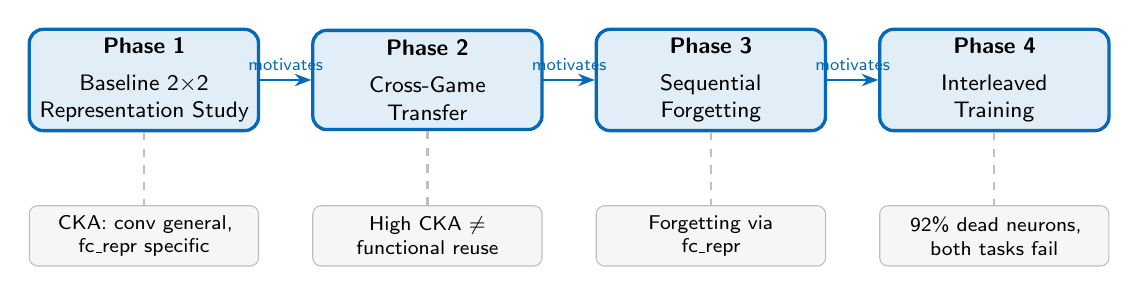
\begin{tikzpicture}[transform shape, scale=0.9,
    phase/.style={
        rectangle, draw=tcdBlue, fill=tcdBlue!12, rounded corners=5pt,
        minimum width=3.2cm, minimum height=1.4cm, text centered,
        text width=3.0cm, line width=1.2pt, font=\small
    },
    finding/.style={
        rectangle, draw=gray!50, fill=gray!7, rounded corners=3pt,
        minimum width=3.2cm, minimum height=0.85cm, text centered,
        text width=3.0cm, font=\footnotesize
    },
    arr/.style={-{Stealth[length=6pt]}, thick, tcdBlue},
    darr/.style={dashed, thick, gray!50}
]

\node[phase] (p1) at (0,0)   {\textbf{Phase 1}\\[4pt]Baseline 2$\times$2\\Representation Study};
\node[phase] (p2) at (4,0)   {\textbf{Phase 2}\\[4pt]Cross-Game\\Transfer};
\node[phase] (p3) at (8,0)   {\textbf{Phase 3}\\[4pt]Sequential\\Forgetting};
\node[phase] (p4) at (12,0)  {\textbf{Phase 4}\\[4pt]Interleaved\\Training};

\node[finding] (f1) at (0,-2.2)  {CKA: conv general,\\fc\_repr specific};
\node[finding] (f2) at (4,-2.2)  {High CKA $\neq$\\functional reuse};
\node[finding] (f3) at (8,-2.2)  {Forgetting via\\fc\_repr};
\node[finding] (f4) at (12,-2.2) {92\% dead neurons,\\both tasks fail};

\draw[arr] (p1) -- node[above, font=\scriptsize, text=tcdBlue]{motivates} (p2);
\draw[arr] (p2) -- node[above, font=\scriptsize, text=tcdBlue]{motivates} (p3);
\draw[arr] (p3) -- node[above, font=\scriptsize, text=tcdBlue]{motivates} (p4);

\draw[darr] (p1.south) -- (f1.north);
\draw[darr] (p2.south) -- (f2.north);
\draw[darr] (p3.south) -- (f3.north);
\draw[darr] (p4.south) -- (f4.north);

\end{tikzpicture}
\caption{Four-phase experimental design. Each phase is motivated by the key finding of
the previous one. CKA analysis (Phase~1) establishes which layers are game-specific;
transfer experiments (Phase~2) test whether geometric similarity implies functional
reusability; sequential forgetting experiments (Phase~3) confirm where forgetting
propagates; and interleaved training (Phase~4) tests whether joint training avoids it.}
\label{fig:overview}
\end{figure}

% ============================================================
\section{Background}
\label{sec:background}
% ============================================================

\subsection{Deep Q-Networks}

DQN \cite{mnih2015human} approximates the action-value function $Q(s, a)$ using a
convolutional neural network. Two mechanisms stabilise training on raw pixel inputs:
experience replay, which stores transitions in a buffer and samples them randomly to break
temporal correlations; and a target network, a periodically frozen copy of the online
network used to compute training targets. The DQN TD target is:

\begin{equation}
    y = r + \gamma \cdot \max_{a'} Q(s', a';\, \theta^{-})
\end{equation}

where $\theta^{-}$ are the target network parameters. Because the same network both selects
and evaluates the best next action, taking the maximum over noisy Q-value estimates produces
a systematic upward bias that compounds over training.

\subsection{Double DQN}

Van Hasselt et al.\ \cite{van2016deep} proposed using the online network to select the
best next action and the target network to evaluate it:

\begin{equation}
    y = r + \gamma \cdot Q\!\left(s',\, \argmax_{a'} Q(s', a';\, \theta);\, \theta^{-}\right)
\end{equation}

Because the two networks have different error profiles, their errors are unlikely to
compound in the same direction, substantially reducing overestimation bias. In this study's
codebase, \texttt{DoubleDQNAgent} inherits everything from \texttt{DQNAgent} and overrides
only the \texttt{learn()} method. Any representational difference between the two agents is
attributable solely to this target formulation.

\subsection{Representation Learning and Capacity Loss}

The 512-dimensional activation vector at the penultimate fully connected layer serves as the
agent's compressed encoding of the current game state. Zahavy et al.\ \cite{zahavy2016graying}
showed that t-SNE projections of DQN representations reveal semantically meaningful
clustering that reflects the underlying value structure of the game rather than raw visual
similarity. Yosinski et al.\ \cite{yosinski2014transferable} demonstrated in supervised
settings that early convolutional layers learn highly general, transferable features while
deeper layers specialise to the training task, a pattern this study tests in the RL domain.

Capacity loss in deep RL refers to the progressive reduction in a network's effective
representational capacity over training. Sokar et al.\ \cite{sokar2023dormant} formally
characterised the dormant neuron phenomenon: neurons whose activations fall chronically near
zero under ReLU, contributing negligibly to the network's computations. They attributed this
to the non-stationary target values inherent in value-based RL, which subject neurons to
conflicting gradient signals until their pre-activation distributions drift permanently
negative. Lyle et al.\ \cite{lyle2022understanding,lyle2023plasticity} deepened this
picture by showing that plasticity loss occurs even in networks with few dead neurons, and
is more fundamentally tied to rank collapse of the Neural Tangent Kernel Gram matrix and
decay of gradient magnitudes. Dead neurons are therefore a reliable indicator of capacity
collapse, but not its sole cause.

\subsection{Catastrophic Forgetting and Continual Learning}

Catastrophic forgetting \cite{mccloskey1989catastrophic} refers to the abrupt loss of
previously learned information when a neural network is trained on a new task. A thorough
treatment of RL foundations and the Bellman optimality conditions underlying these algorithms
is given in Sutton and Barto \cite{sutton2018reinforcement}. In deep RL, the forgetting
problem is compounded by non-stationarity: unlike supervised learning, where the data
distribution is fixed, value-based RL targets shift continuously as the policy improves,
creating a more volatile gradient landscape throughout training. Igl et al.\ \cite{igl2021transient}
showed that early exposure to this non-stationary signal leaves a lasting geometric imprint
on the representation space that degrades generalisation even after the data distribution
stabilises.

Standard mitigations include Elastic Weight Consolidation \cite{kirkpatrick2017overcoming},
which penalises changes to weights important for the original task; progressive networks
\cite{rusu2016progressive}, which freeze old networks entirely and grow lateral connections
for new tasks; and continual backpropagation \cite{elsayed2024continual,dohare2024loss},
which periodically reinitialises low-utility neurons to maintain plasticity. This study
focuses on a simpler and more interpretable intervention: layer freezing guided by the CKA
analysis of which layers are general versus game-specific.

\subsection{Multi-Task Gradient Interference}

When a shared network is trained on multiple tasks simultaneously, gradients from different
tasks can point in conflicting directions. If the cosine similarity between two task
gradients is negative, applying the average update degrades both tasks rather than
improving them. Yu et al.\ \cite{yu2020pcgrad} formalised this as gradient interference
and showed it is common in multi-task settings with structurally different objectives.
Elhage et al.\ \cite{elhage2022superposition} provided a complementary perspective through
the concept of superposition: networks with limited representational capacity are forced to
encode multiple features in overlapping subspaces when the total feature load exceeds
available dimensions, with ReLU saturation serving as the network's mechanism for silencing
unresolvable interference.

\subsection{Centred Kernel Alignment}

Centred Kernel Alignment (CKA) \cite{kornblith2019similarity} measures the similarity
between two sets of representations, independent of linear transformations. Given activation
matrices $X \in \mathbb{R}^{n \times p}$ and $Y \in \mathbb{R}^{n \times q}$ collected
over the same $n$ inputs:

\begin{equation}
    \text{CKA}(X, Y) = \frac{\|Y^{\top}X\|_F^2}{\|X^{\top}X\|_F \cdot \|Y^{\top}Y\|_F}
\end{equation}

CKA returns values in $[0, 1]$, where 1 indicates identical representational geometry up
to linear transformation. Both networks must be evaluated on the same inputs for CKA to be
meaningful; using different game states per network would measure input dissimilarity rather
than representational similarity.

\subsection{t-SNE and Grad-CAM}

t-SNE \cite{van2008visualizing} reduces high-dimensional data to two dimensions by
minimising the KL divergence between Gaussian neighbourhood distributions in the original
space and Student-t distributions in the 2D projection, faithfully preserving local cluster
structure. Grad-CAM \cite{selvaraju2017grad} produces visual explanations by backpropagating
gradients to the final convolutional layer and weighting feature maps by their importance
to the output.

% ============================================================
\section{Experimental Design}
\label{sec:method}
% ============================================================

\subsection{Factorial Baseline}

The study uses a fully crossed 2$\times$2 factorial design, crossing algorithm (DQN, DDQN)
with game (Pong, Breakout), as summarised in Table~\ref{tab:factorial}:

\begin{table}[H]
\centering
\caption{Factorial design. All four runs use identical hyperparameters and the same random seed.}
\label{tab:factorial}
\begin{tabular}{lcc}
\toprule
 & \textbf{Pong} & \textbf{Breakout} \\
\midrule
\textbf{DQN}  & Run 1 (2M steps) & Run 2 (5M steps) \\
\textbf{DDQN} & Run 3 (2M steps) & Run 4 (5M steps) \\
\bottomrule
\end{tabular}
\end{table}

\subsection{Preprocessing and Architecture}

Raw 210$\times$160 RGB frames from the Arcade Learning Environment \cite{bellemare2013arcade}
are transformed through the standard DeepMind preprocessing stack \cite{mnih2015human}:
no-op reset, frame skip (4), episodic life, grayscale and resize to 84$\times$84, reward
clipping to $\{-1, 0, +1\}$, and frame stacking (4 frames).

Hyperparameters are listed in Table~\ref{tab:hyperparams}. Both agents share the CNN from
Mnih et al.: three convolutional layers (32 filters, 8$\times$8, stride 4; 64 filters,
4$\times$4, stride 2; 64 filters, 3$\times$3, stride 1),
followed by a 512-dimensional fully connected representation layer (\texttt{fc\_repr}) with
ReLU activation, and a linear output head (\texttt{fc\_out}) producing Q-values for each
action. A PyTorch forward hook on \texttt{fc\_repr} captures the 512-dim activation after
every forward pass without modifying computation. Weights use orthogonal
initialisation \cite{saxe2013exact}. The full architecture is illustrated in
Figure~\ref{fig:architecture}.

\begin{figure}[H]
\centering
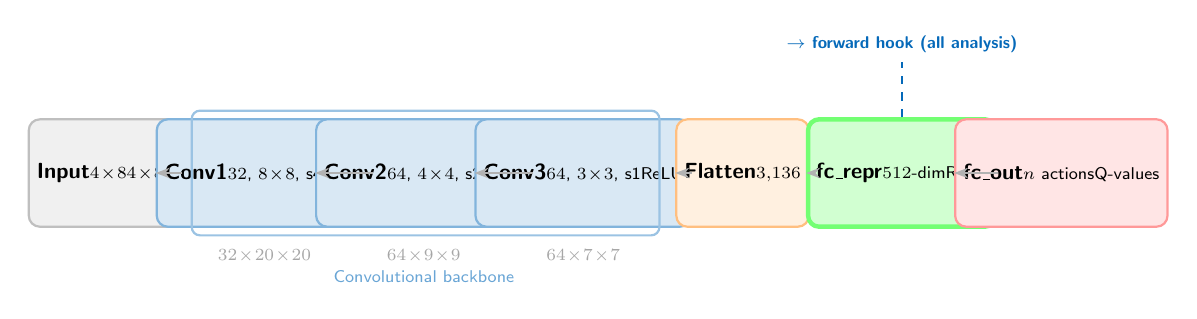
\begin{tikzpicture}[
    transform shape, scale=0.88,
    every node/.style={font=\small},
    box/.style={
        rectangle, rounded corners=4pt, draw, thick,
        minimum width=1.85cm, minimum height=1.55cm, text centered
    },
    arr/.style={-{Stealth[length=5pt]}, thick, gray!60}
]

%% ---- Layer nodes ----
\node[box, fill=gray!12,     draw=gray!50]  (inp)   at (0,0)    {\textbf{Input}\\[3pt]\scriptsize$4\!\times\!84\!\times\!84$};
\node[box, fill=tcdBlue!15,  draw=tcdBlue!50] (c1) at (2.3,0)  {\textbf{Conv1}\\[3pt]\scriptsize$32$, $8\!\times\!8$, s4\\[1pt]\scriptsize ReLU};
\node[box, fill=tcdBlue!15,  draw=tcdBlue!50] (c2) at (4.6,0)  {\textbf{Conv2}\\[3pt]\scriptsize$64$, $4\!\times\!4$, s2\\[1pt]\scriptsize ReLU};
\node[box, fill=tcdBlue!15,  draw=tcdBlue!50] (c3) at (6.9,0)  {\textbf{Conv3}\\[3pt]\scriptsize$64$, $3\!\times\!3$, s1\\[1pt]\scriptsize ReLU};
\node[box, fill=orange!12,   draw=orange!50] (fl)  at (9.2,0)  {\textbf{Flatten}\\[3pt]\scriptsize$3{,}136$};
\node[box, fill=green!18,    draw=green!55, ultra thick] (fc) at (11.5,0) {\textbf{fc\_repr}\\[3pt]\scriptsize$512$-dim\\[1pt]\scriptsize ReLU};
\node[box, fill=red!10,      draw=red!40]   (out) at (13.8,0)  {\textbf{fc\_out}\\[3pt]\scriptsize$n$ actions\\[1pt]\scriptsize Q-values};

%% ---- Arrows ----
\draw[arr] (inp) -- (c1);
\draw[arr] (c1)  -- (c2);
\draw[arr] (c2)  -- (c3);
\draw[arr] (c3)  -- (fl);
\draw[arr] (fl)  -- (fc);
\draw[arr] (fc)  -- (out);

%% ---- Output sizes below conv nodes ----
\node[font=\scriptsize, text=gray!70] at (2.3,-1.2)  {$32\!\times\!20\!\times\!20$};
\node[font=\scriptsize, text=gray!70] at (4.6,-1.2)  {$64\!\times\!9\!\times\!9$};
\node[font=\scriptsize, text=gray!70] at (6.9,-1.2)  {$64\!\times\!7\!\times\!7$};

%% ---- Forward hook annotation ----
\draw[dashed, tcdBlue, thick] (fc.north) -- ++(0, 0.8)
    node[above, font=\scriptsize\bfseries, text=tcdBlue]
    {$\rightarrow$ forward hook (all analysis)};

%% ---- Backbone bracket ----
\draw[tcdBlue!40, thick, rounded corners=3pt]
    (1.25, -0.9) rectangle (8.0, 0.9);
\node[font=\scriptsize, text=tcdBlue!60] at (4.6, -1.5)
    {Convolutional backbone};

\end{tikzpicture}
\caption{CNN architecture shared by all agents. The three blue convolutional layers form
the backbone. The green \texttt{fc\_repr} layer (512-dim, marked with a forward hook) is
where all representation analysis is performed. The \texttt{fc\_out} head is game-specific
(Pong: 6 actions; Breakout: 4 actions). Feature map sizes after each conv layer are shown
below the nodes. Approximately 95\% of the ${\sim}1.7$M total parameters reside in
\texttt{fc\_repr}.}
\label{fig:architecture}
\end{figure}

\begin{table}[H]
\centering
\caption{Hyperparameters used across all runs.}
\label{tab:hyperparams}
\begin{tabularx}{\linewidth}{lX}
\toprule
\textbf{Parameter} & \textbf{Value} \\
\midrule
Learning rate            & $1 \times 10^{-4}$ (Adam) \\
Replay buffer            & 100,000 transitions \\
Batch size               & 32 \\
Discount factor $\gamma$ & 0.99 \\
Target update frequency  & 1,000 steps (hard copy) \\
Epsilon schedule         & $1.0 \to 0.01$ over 100,000 steps \\
Gradient clipping        & $L_2$ norm $\leq 10.0$ \\
Checkpoint frequency     & Every 500,000 steps \\
Random seed              & 42 \\
\bottomrule
\end{tabularx}
\end{table}

\subsection{CKA Layer Analysis}

Forward hooks are registered at conv1, conv2, conv3, and fc\_repr. Activations are collected
by running all four agents on 1,000 shared Pong frames obtained via random actions. Using
random actions ensures a diverse, policy-neutral probe of the state space, and the shared
frame set is essential for CKA validity: both networks must process the same inputs for the
similarity measure to reflect representational geometry rather than input differences.

\subsection{Cross-Game Transfer Experiments}

\textbf{Zero-shot evaluation.} Chimera networks are constructed by transplanting
convolutional layers from one trained agent into another game's upper layers, with no
additional training. Ten conditions are evaluated across both games (50 episodes each),
spanning native agents through cross-game and cross-algorithm chimeras to fully random
networks.

\textbf{Backbone training.} DQN is initialised from the converged DQN/Pong checkpoint and
trained on Breakout for 5M steps under three conditions: scratch (random initialisation
baseline), frozen conv (Pong conv layers locked), and full fine-tune (all layers initialised
from Pong, all trainable).

\subsection{Sequential Training and Forgetting Measurement}

Three conditions test catastrophic forgetting when a trained Pong agent continues training
on Breakout for 2M steps:

\textbf{No freeze.} All layers adapt freely. Serves as the forgetting baseline.

\textbf{Freeze conv.} Conv layers are frozen; fc\_repr and a new Breakout output head train.
This tests whether freezing only the convolutional layers, which CKA identifies as the most
general, is sufficient to protect Pong performance.

\textbf{Freeze all.} Conv layers and fc\_repr are both loaded from Pong and frozen. Only a
new Breakout output head (512$\times$4 = 2,052 parameters) trains. This tests whether
freezing the full backbone prevents forgetting.

Forgetting is measured every 200,000 Breakout training steps via three signals: (1) Pong
reward, evaluated using a chimera network composed of the current backbone with the original
Pong output head; (2) dead neuron fraction in fc\_repr; and (3) CKA drift, the similarity
between current fc\_repr activations and the original Pong fc\_repr activations on a fixed
set of Pong frames.

\subsection{Interleaved Training}

A single DQN agent with a shared backbone (\texttt{conv1}--\texttt{conv3} + \texttt{fc\_repr})
and two game-specific output heads trains from random initialisation on both Pong and
Breakout simultaneously. Rather than alternating at the episode level, which would create a
severe gradient imbalance due to Pong episodes averaging roughly 200 steps while Breakout
episodes (with episodic life wrappers) average approximately 10, the agent switches active
game every 1,000 environment steps. This step-level alternation ensures exactly equal
gradient contribution from both games regardless of episode length asymmetry, with each
game receiving 1M total training steps over the 2M step run.

Separate replay buffers are maintained per game to prevent cross-contamination of
experience. The epsilon schedule decays over 200,000 steps rather than 100,000 to account
for the larger effective training horizon with two simultaneous tasks. The same forgetting
metrics used in the sequential experiments (Pong reward, dead neuron fraction, CKA drift)
are recorded every 100,000 total steps, enabling direct comparison with sequential
conditions.

% ============================================================
\section{Results}
\label{sec:results}
% ============================================================

\subsection{Training Performance}

\begin{table}[H]
\centering
\caption{Training results for all four baseline agents. Reward statistics over the final 50 episodes.}
\label{tab:results}
\begin{tabularx}{\linewidth}{lXXXX}
\toprule
\textbf{Agent} & \textbf{Episodes} & \textbf{Final Reward} & \textbf{Final Q} & \textbf{Peak Q} \\
\midrule
DQN / Pong      & 2,434   & $7.12 \pm 5.22$ & 2.64 & 2.95 \\
DDQN / Pong     & 2,457   & $7.50 \pm 5.03$ & 2.05 & 2.48 \\
DQN / Breakout  & 144,751 & $3.86 \pm 4.94$ & 4.06 & 5.39 \\
DDQN / Breakout & 144,948 & $4.00 \pm 5.04$ & 4.13 & 4.55 \\
\bottomrule
\end{tabularx}
\end{table}

Both algorithms reach comparable final reward on both games (Table~\ref{tab:results},
Figure~\ref{fig:training_curves}). On Pong, DQN achieves $7.12 \pm 5.22$ and DDQN
$7.50 \pm 5.03$. On Breakout, DQN reaches $3.86 \pm 4.94$ and DDQN $4.00 \pm 5.04$.
The near-identical task performance is important: any representational differences observed
in subsequent analysis cannot be attributed to differences in what the agents learned to
do, only to differences in how they represent it internally.

\begin{figure}[H]
    \centering
    \begin{subfigure}[b]{0.48\linewidth}
        
\includegraphics[width=\linewidth]{figures/training_curves_pong.png}
        \caption{Pong.}
    \end{subfigure}
    \hfill
    \begin{subfigure}[b]{0.48\linewidth}
        
\includegraphics[width=\linewidth]{figures/training_curves_breakout.png}
        \caption{Breakout.}
    \end{subfigure}
    \caption{Training curves (20-episode rolling average). Both algorithms reach comparable
    final reward on both games.}
    \label{fig:training_curves}
\end{figure}

\subsection{Q-Value Overestimation}

DQN Q-values on Pong peak at 2.95 and settle at 2.64; DDQN peaks at 2.48 and settles at
2.05, approximately 29\% lower (Figure~\ref{fig:qvalue}). On Breakout the gap is smaller, with DQN showing a higher
peak (5.39 versus 4.55) consistent with overestimation being amplified during the most
uncertain phases of early training. These inflated Q-values are not merely a measurement
artefact: they reflect genuinely higher-variance gradient signals propagating back through
the network, which has downstream consequences for the quality and stability of the
representations DDQN and DQN develop.

\begin{figure}[H]
    \centering
    
\includegraphics[width=0.7\linewidth]{figures/qvalue_overestimation.png}
    \caption{Mean maximum Q-value over training. DQN values drift upward; DDQN values
    remain lower and more stable throughout.}
    \label{fig:qvalue}
\end{figure}

\subsection{t-SNE Representation Analysis}

The dominant structural feature of the t-SNE embeddings is separation by game. When all
four agents are projected together, two primary clusters emerge corresponding to Pong and
Breakout, with algorithm-level sub-structure visible within each (Figure~\ref{fig:all_agents}).
Game separation is consistent across both algorithms (Figure~\ref{fig:game_effect}): the
game played is the primary organising principle of the representation space; the algorithm
used is secondary.

\begin{figure}[H]
    \centering
    \begin{subfigure}[b]{0.48\linewidth}
        
\includegraphics[width=\linewidth]{figures/tsne_game_effect_dqn.png}
        \caption{DQN: Pong vs Breakout.}
    \end{subfigure}
    \hfill
    \begin{subfigure}[b]{0.48\linewidth}
        
\includegraphics[width=\linewidth]{figures/tsne_game_effect_ddqn.png}
        \caption{DDQN: Pong vs Breakout.}
    \end{subfigure}
    \caption{Game effect: representations separate cleanly by game regardless of algorithm.}
    \label{fig:game_effect}
\end{figure}

Within each game, DDQN produces tighter cluster geometry with lower intra-cluster spread
(Figure~\ref{fig:algo_effect}). To quantify this, we compute the mean Euclidean distance
from each agent's representation centroid over 1,000 sampled states. DDQN/Pong has a mean
centroid distance of 4.65 (DQN/Pong: 5.07); DDQN/Breakout has 7.42 (DQN/Breakout: 7.60).
The gap is most pronounced in cosine distance: DDQN/Breakout shows a mean intra-cluster
cosine distance of 0.328 versus 0.416 for DQN/Breakout, a 21\% reduction. On Pong the
cosine gap is smaller and in the opposite direction (DQN/Pong: 0.231, DDQN/Pong: 0.280),
suggesting DDQN's tighter geometry is more consistent on the harder game. Game separation
silhouette scores are similar across algorithms (DQN: 0.49, DDQN: 0.50), confirming that
the game effect dominates equally for both. Table~\ref{tab:cluster} summarises these
cluster statistics.

\begin{table}[H]
\centering
\caption{Quantitative cluster statistics for fc\_repr representations (1,000 sampled
states per agent). Mean centroid distance and mean pairwise cosine distance measure
intra-cluster spread (lower = tighter). Game separation silhouette measures how cleanly
Pong and Breakout clusters separate (higher = more separated; computed on PCA-50 projections).}
\label{tab:cluster}
\begin{tabular}{lccc}
\toprule
\textbf{Agent} & \textbf{Centroid dist.} & \textbf{Intra cosine dist.} & \textbf{Game sep. silhouette} \\
\midrule
DQN / Pong      & 5.07 & 0.231 & 0.49 \\
DDQN / Pong     & \textbf{4.65} & 0.280 & 0.50 \\
DQN / Breakout  & 7.60 & 0.416 & 0.49 \\
DDQN / Breakout & \textbf{7.42} & \textbf{0.328} & 0.50 \\
\bottomrule
\end{tabular}
\end{table}

\begin{figure}[H]
    \centering
    \begin{subfigure}[b]{0.48\linewidth}
        
\includegraphics[width=\linewidth]{figures/tsne_algo_effect_pong.png}
        \caption{Algorithm effect on Pong.}
    \end{subfigure}
    \hfill
    \begin{subfigure}[b]{0.48\linewidth}
        
\includegraphics[width=\linewidth]{figures/tsne_algo_effect_breakout.png}
        \caption{Algorithm effect on Breakout.}
    \end{subfigure}
    \caption{Algorithm effect: DDQN produces tighter cluster geometry within each game.}
    \label{fig:algo_effect}
\end{figure}

\begin{figure}[H]
    \centering
    
\includegraphics[width=0.6\linewidth]{figures/tsne_all_agents.png}
    \caption{All four agents. Game clusters dominate; algorithm sub-structure is visible
    within each.}
    \label{fig:all_agents}
\end{figure}

Representations coloured by episode reward show a partial spatial correspondence between
t-SNE position and value, more consistently under DDQN (Figure~\ref{fig:reward}). Temporal
evolution plots (Figure~\ref{fig:temporal}) show representations beginning as diffuse clouds
and tightening progressively over training, with DDQN developing distinct structure earlier
on both games.

\begin{figure}[H]
    \centering
    
\includegraphics[width=0.65\linewidth]{figures/tsne_by_reward.png}
    \caption{t-SNE coloured by cumulative reward. Spatial correspondence between value and
    position is more consistent under DDQN.}
    \label{fig:reward}
\end{figure}

\begin{figure}[H]
    \centering
    \begin{subfigure}[b]{0.48\linewidth}
        
\includegraphics[width=\linewidth]{figures/tsne_temporal_dqn_pong.png}
        \caption{DQN / Pong.}
    \end{subfigure}
    \hfill
    \begin{subfigure}[b]{0.48\linewidth}
        
\includegraphics[width=\linewidth]{figures/tsne_temporal_ddqn_pong.png}
        \caption{DDQN / Pong.}
    \end{subfigure}
    \vskip\baselineskip
    \begin{subfigure}[b]{0.48\linewidth}
        
\includegraphics[width=\linewidth]{figures/tsne_temporal_dqn_breakout.png}
        \caption{DQN / Breakout.}
    \end{subfigure}
    \hfill
    \begin{subfigure}[b]{0.48\linewidth}
        
\includegraphics[width=\linewidth]{figures/tsne_temporal_ddqn_breakout.png}
        \caption{DDQN / Breakout.}
    \end{subfigure}
    \caption{Temporal evolution across all four agents. Representations tighten over
    training; DDQN develops structure earlier on both games.}
    \label{fig:temporal}
\end{figure}

\subsection{Saliency Maps}

Grad-CAM maps reveal consistent attention across all four agents: the ball attracts the
highest saliency, with secondary attention on the agent's own paddle. DDQN saliency is more
spatially concentrated than DQN on both games, and shows greater forward-looking attention
toward bricks in the ball's trajectory on Breakout (Figures~\ref{fig:saliency_pong}
and~\ref{fig:saliency_breakout}).

\begin{figure}[H]
    \centering
    
\includegraphics[width=0.7\linewidth]{figures/saliency_pong.png}
    \caption{Grad-CAM saliency on Pong. Both agents attend to the ball; DDQN attention is
    more spatially concentrated.}
    \label{fig:saliency_pong}
\end{figure}

\begin{figure}[H]
    \centering
    
\includegraphics[width=0.7\linewidth]{figures/saliency_breakout.png}
    \caption{Grad-CAM saliency on Breakout. DDQN shows more focused attention on the ball
    and bricks in its path.}
    \label{fig:saliency_breakout}
\end{figure}

\subsection{Dead Neurons and Cosine Similarity}

Dead neurons (those firing in fewer than 5\% of game states) are consistently higher under
DQN than DDQN across both games (Figure~\ref{fig:dead_neurons}). This is consistent with
DQN's higher-variance gradient signal accelerating the saturation of ReLU units, as
characterised by Sokar et al.\ \cite{sokar2023dormant}.

A notable feature of Table~\ref{tab:sequential} is that the successfully trained Pong agent
already has a dead neuron fraction of approximately 0.879 before any Breakout training begins.
This high baseline is itself a finding consistent with the literature: Sokar et al.\ showed
that single-task DQN agents routinely accumulate large dormant fractions during training as a
consequence of non-stationary TD targets. Importantly, the agent still achieves a mean reward
of $+9.1$ despite only roughly 63 of its 512 fc\_repr neurons being meaningfully active, which
suggests the architecture is over-parameterised relative to what Pong requires, and that the
remaining active neurons encode a sufficiently rich policy. This baseline context matters for
interpreting the capacity collapse observed in later experiments: the capacity available to
encode a second game is not 512 neurons but far fewer, making gradient interference between
two tasks substantially more acute than the raw architecture size would imply.

Cross-game cosine similarity is non-trivial for both algorithms, with DDQN showing marginally
higher alignment (Figure~\ref{fig:cosine}), suggesting its representations preserve more of the
shared visual content that Pong and Breakout genuinely have in common.

\begin{figure}[H]
    \centering
    
\includegraphics[width=0.7\linewidth]{figures/dead_neurons.png}
    \caption{Dead neuron fraction over training. DQN consistently develops more inactive
    neurons than DDQN.}
    \label{fig:dead_neurons}
\end{figure}

\begin{figure}[H]
    \centering
    
\includegraphics[width=0.7\linewidth]{figures/cosine_similarity.png}
    \caption{Cross-game cosine similarity. DDQN shows higher alignment, consistent with
    less gradient noise in its learned features.}
    \label{fig:cosine}
\end{figure}

\subsection{Layer-wise CKA Similarity}

CKA is computed between the Pong and Breakout agents at each of four layer depths using
1,000 shared Pong frames (Figure~\ref{fig:cka}). The shared frame set is essential: running
each network on its own game's frames would measure input dissimilarity rather than
representational similarity.

\begin{figure}[H]
    \centering
    
\includegraphics[width=0.7\linewidth]{figures/layer_similarity_cka.png}
    \caption{Layer-wise CKA between Pong and Breakout agents. High similarity at early conv
    layers drops sharply at fc\_repr.}
    \label{fig:cka}
\end{figure}

Table~\ref{tab:cka} reports the full CKA matrix. Under DDQN, cross-game CKA is 0.92 at
conv1, 0.85 at conv2, 0.41 at conv3, and just 0.09 at fc\_repr, a tenfold drop from early
to late layers.

\begin{table}[H]
\centering
\caption{Layer-wise CKA similarity at four network depths. \emph{Game effect} compares
Pong vs Breakout within the same algorithm. \emph{Algorithm effect} compares DQN vs DDQN
on the same game. All values computed on 1,000 shared Pong probe frames.}
\label{tab:cka}
\begin{tabular}{lcccc}
\toprule
\textbf{Layer} & \textbf{Game (DQN)} & \textbf{Game (DDQN)} & \textbf{Algo (Pong)} & \textbf{Algo (Breakout)} \\
\midrule
conv1   & 0.67 & 0.90 & 0.998 & 0.75 \\
conv2   & 0.73 & 0.85 & 0.96  & 0.73 \\
conv3   & 0.40 & 0.41 & 0.87  & 0.57 \\
fc\_repr & 0.05 & 0.09 & 0.56  & 0.46 \\
\bottomrule
\end{tabular}
\end{table} The pattern holds under DQN (0.68,
0.72, 0.40, 0.05). Algorithm-effect comparisons within the same game show much higher
similarity at all depths: on Pong, conv1 = 0.998, conv2 = 0.96, conv3 = 0.87, fc\_repr =
0.56, confirming that both algorithms develop functionally near-identical visual processing
pipelines for the same game while differing in representational quality. The sharpest drop
in game-effect CKA occurs between conv3 and fc\_repr, falling from approximately 0.40 to
0.07. This marks the layer at which the network transitions from pixel-level feature
extraction to state-value encoding, where game-specific strategic demands take over from
general visual processing.

\subsection{Cross-Game Transfer}

\subsubsection{Zero-Shot Evaluation}

\begin{figure}[H]
    \centering
    \begin{subfigure}[b]{0.48\linewidth}
        
\includegraphics[width=\linewidth]{figures/mix_and_match_breakout.png}
        \caption{Evaluated on Breakout.}
    \end{subfigure}
    \hfill
    \begin{subfigure}[b]{0.48\linewidth}
        
\includegraphics[width=\linewidth]{figures/mix_and_match_pong.png}
        \caption{Evaluated on Pong.}
    \end{subfigure}
    \caption{Zero-shot mix-and-match evaluation. Transplanting conv layers produces
    performance equivalent to random initialisation.}
    \label{fig:mixmatch}
\end{figure}

On Breakout, DQN/Pong conv transplanted into a DQN/Breakout agent achieves $0.44 \pm 0.78$,
compared to $0.40 \pm 1.00$ for random conv and $0.42 \pm 0.80$ for a fully random network.
The native agent scores $3.40 \pm 3.82$ (Figure~\ref{fig:mixmatch}). On Pong, any foreign conv layer, whether from
Breakout, a different algorithm, or random initialisation, produces a score of $-21$, the
worst possible. High CKA at conv layers does not translate to functional compatibility:
fc\_repr was trained to interpret its own conv stack's specific activation patterns, and
foreign conv activations, even if geometrically similar, fall outside that trained
distribution and produce meaningless Q-value estimates.

\subsubsection{Backbone Training}

\begin{figure}[H]
    \centering
    
\includegraphics[width=0.85\linewidth]{figures/backbone_comparison_reward.png}
    \caption{Breakout learning curves: scratch DQN vs frozen Pong conv vs full fine-tune
    from Pong. 500-episode rolling average.}
    \label{fig:backbone}
\end{figure}

\begin{figure}[H]
    \centering
    
\includegraphics[width=0.85\linewidth]{figures/backbone_comparison_qvalue.png}
    \caption{Q-value trajectories for the three backbone conditions. Full fine-tune shows
    higher peak Q-values consistent with the Pong warm start; frozen conv Q-values remain
    suppressed, reflecting limited representational adaptation.}
    \label{fig:backbone_qvalue}
\end{figure}

\begin{table}[H]
\centering
\caption{Backbone training results on Breakout after 5M steps.}
\label{tab:backbone}
\begin{tabular}{lcc}
\toprule
\textbf{Condition} & \textbf{Final Reward} & \textbf{Best Smoothed} \\
\midrule
Scratch                   & 3.86 & 4.07 \\
Frozen conv (Pong)        & 2.28 & 3.03 \\
Full fine-tune from Pong  & 3.12 & 4.47 \\
\bottomrule
\end{tabular}
\end{table}

Frozen Pong conv underperforms scratch throughout training (Table~\ref{tab:backbone},
Figures~\ref{fig:backbone} and~\ref{fig:backbone_qvalue}), despite CKA showing those layers
are geometrically similar to what Breakout would develop independently. Pong's conv layers
encode features that are reward-predictive in Pong's visual context, such as opponent paddle
trajectories and approaching ball angles, which differ subtly from the features most useful
for Breakout. Freezing them constrains rather than accelerates Breakout learning. Full
fine-tune from Pong initialisation achieves the highest peak (4.47 smoothed), suggesting
Pong weights provide a useful warm start when all layers can subsequently adapt freely.

\subsection{Sequential Training: Catastrophic Forgetting}

Figure~\ref{fig:forgetting} shows the three forgetting metrics over 2M Breakout training
steps for all conditions, including the interleaved result described in the following
subsection.

\begin{figure}[H]
    \centering
    
\includegraphics[width=\linewidth]{figures/forgetting_curves.png}
    \caption{Forgetting curves across all conditions. Left: Pong reward. Centre: dead neuron
    fraction. Right: CKA drift from original Pong representations. Freeze-all maintains Pong
    performance throughout; interleaved training produces the worst outcome.}
    \label{fig:forgetting}
\end{figure}

\begin{table}[H]
\centering
\caption{Sequential training results. Pong reward, dead neurons, and CKA drift at start
(step 0) and end (step 2M) of Breakout training.}
\label{tab:sequential}
\begin{tabularx}{\linewidth}{lXXXXXX}
\toprule
 & \multicolumn{2}{c}{\textbf{Pong Reward}} & \multicolumn{2}{c}{\textbf{Dead Neurons}} & \multicolumn{2}{c}{\textbf{CKA Drift}} \\
\cmidrule(lr){2-3}\cmidrule(lr){4-5}\cmidrule(lr){6-7}
\textbf{Condition} & Step 0 & Step 2M & Step 0 & Step 2M & Step 0 & Step 2M \\
\midrule
No freeze     & 9.1 & $-$20.8 & 0.879 & 0.873 & 0.037 & 0.041 \\
Freeze conv   & 9.1 & $-$14.0 & 0.879 & 0.836 & 0.055 & 0.043 \\
Freeze all    & 9.1 & \ \ \ 9.4  & 0.877 & 0.881 & 0.035 & 0.065 \\
\bottomrule
\end{tabularx}
\end{table}

\textbf{No freeze.} Pong reward collapses from $+9.1$ to $-20.75$ within the first 200,000
Breakout training steps and never recovers, reaching $-20.8$ at 2M steps. The collapse is
essentially instantaneous on the scale of the experiment: one tenth of the way through
Breakout training, Pong performance is already at its floor. Dead neurons rise and then
partially recover as the network stabilises on its new task.

\textbf{Freeze conv.} Pong reward degrades more gradually but still substantially, falling
to $-3.75$ by 200k steps and continuing to $-14.0$ at 2M steps. Freezing only the
convolutional layers is insufficient to prevent forgetting because fc\_repr continues to
adapt freely to Breakout's strategic demands, progressively destroying the Pong-specific
value encoding it had developed.

\textbf{Freeze all.} Pong reward remains stable throughout training, fluctuating between
7.2 and 10.65 across all evaluation points and ending at 9.4 after 2M Breakout steps.
Freezing both conv layers and fc\_repr preserves the full Pong policy pathway almost
completely. The result is that a network trained on only 2,052 parameters (the new Breakout
output head) can begin learning Breakout while leaving Pong intact.

A methodological note on the CKA drift values: the probe procedure collects representations
by stepping through the Pong environment with random actions, but the action space random
state is not fixed between evaluations. Successive evaluations therefore sample different
state distributions, and CKA between two collections from the same frozen network falls
below 1.0. The freeze-all values (0.035 to 0.065) lie within this measurement floor and
should be read as consistent with zero structural change rather than as evidence of genuine
representational drift. A more reliable implementation would fix the probe state set by
collecting and saving frames once and reusing them across all evaluations. The no-freeze
and freeze-conv drift values also start near zero for the same reason, meaning the CKA
drift signal is largely masked for all conditions; Pong reward and dead neuron fraction
are the more informative forgetting signals in these experiments.

The connection to the CKA analysis is direct and clean. CKA identified fc\_repr as the
layer with the sharpest cross-game divergence (CKA = 0.09). The sequential experiments
confirm that this is also the layer through which forgetting propagates: when fc\_repr is
free to adapt, Pong performance collapses; when fc\_repr is frozen, Pong performance is
maintained. The forgetting is localised to exactly the layer that CKA predicted would need
to specialise to game-specific strategic demands.

\subsection{Interleaved Training}

\begin{figure}[H]
    \centering
    
\includegraphics[width=\linewidth]{figures/interleaved_curves.png}
    \caption{Interleaved training (step-level alternation, 1M steps per game). Left: Pong
    reward remains at $-21$ throughout. Centre: Breakout reward stays near 0.4 (baseline:
    3.86). Right: dead neuron fraction climbs to 92\%. Dashed lines show standalone
    single-task baselines for comparison.}
    \label{fig:interleaved}
\end{figure}

\begin{table}[H]
\centering
\caption{Interleaved training metrics at key checkpoints. Each game receives exactly half
the total steps at any point.}
\label{tab:interleaved}
\begin{tabularx}{\linewidth}{XXXXXXX}
\toprule
\textbf{Total} & \textbf{Pong} & \textbf{Breakout} & \textbf{Pong} & \textbf{Breakout} & \textbf{Dead} & \textbf{CKA} \\
\textbf{Steps} & \textbf{Steps} & \textbf{Steps} & \textbf{Reward} & \textbf{Reward} & \textbf{Neurons} & \textbf{Drift} \\
\midrule
0       & 0      & 0      & 0.0   & 0.0 & 0.47 & 0.015 \\
200k    & 100k   & 100k   & $-$20.9 & 1.0 & 0.87 & 0.008 \\
500k    & 250k   & 250k   & $-$20.9 & 0.4 & 0.71 & 0.009 \\
1M      & 500k   & 500k   & $-$21.0 & 0.2 & 0.86 & 0.007 \\
2M      & 1M     & 1M     & $-$21.0 & 0.4 & 0.92 & 0.011 \\
\bottomrule
\end{tabularx}
\end{table}

The interleaved results are unambiguous (Table~\ref{tab:interleaved},
Figure~\ref{fig:interleaved}): step-level alternation with equal gradient signal from both
games produces complete failure on both tasks. Pong reward reaches $-21$ within
the first 200,000 total steps and never improves, despite receiving 1M steps of gradient
signal over the full run. Breakout reaches a peak of 0.4, compared to 3.86 when trained
from scratch with the same number of steps. By the end of training, 92.2\% of fc\_repr
neurons are dead, compared to approximately 87\% in single-task training and 87--88\% in
the sequential conditions.

Critically, CKA drift from the Pong baseline remains low throughout (0.007--0.013),
indicating that the shared backbone never moved far from its Pong initialisation geometry.
The network is simultaneously receiving gradient pressure to encode Pong and Breakout
features within the same 512 dimensions, and neither task has sufficient gradient
dominance to drive the representation toward a stable configuration for either game. The
result is a frozen, degraded backbone that is useful for neither.

Comparing all conditions in Table~\ref{tab:comparison}, interleaved training is the worst
outcome, worse than even the no-freeze sequential baseline, which at least succeeds at
Breakout (final reward 3.86) before forgetting Pong.

\begin{table}[H]
\centering
\caption{Comparison of all training conditions. Pong and Breakout reward at the end of
training.}
\label{tab:comparison}
\begin{tabular}{lccc}
\toprule
\textbf{Condition} & \textbf{Pong Final} & \textbf{Breakout Final} & \textbf{Dead Neurons} \\
\midrule
Scratch Breakout        & --      & 3.86 & -- \\
Sequential no freeze    & $-$20.8 & $\sim$3.5 & 0.87 \\
Sequential freeze conv  & $-$14.0 & $\sim$2.5 & 0.84 \\
Sequential freeze all   & $+$9.4  & very limited & 0.88 \\
Interleaved (v2)        & $-$21.0 & 0.4  & \textbf{0.92} \\
\bottomrule
\end{tabular}
\end{table}

\subsection{Results Summary}

Table~\ref{tab:master} consolidates the key quantitative outcomes across all experiments
for a direct cross-condition comparison.

\begin{table}[H]
\centering
\caption{Master results summary across all experimental conditions. Dead neuron fractions
are measured at fc\_repr. n/a indicates the metric is not applicable for that condition.}
\label{tab:master}
\small
\begin{tabular}{lcccc}
\toprule
\textbf{Condition} & \textbf{Pong reward} & \textbf{Breakout reward} & \textbf{Dead neurons} & \textbf{Key finding} \\
\midrule
DQN standalone        & $7.12 \pm 5.22$   & $3.86 \pm 4.94$   & 0.88 (baseline) & Game-specific fc\_repr \\
DDQN standalone       & $7.50 \pm 5.03$   & $4.00 \pm 5.04$   & lower than DQN  & Tighter representations \\
\midrule
Scratch Breakout      & n/a               & 3.86              & n/a             & Transfer baseline \\
Frozen conv (Pong)    & n/a               & 2.28              & n/a             & Conv too task-specific \\
Full fine-tune (Pong) & n/a               & 3.12 (peak 4.47)  & n/a             & Best Breakout peak \\
\midrule
Sequential no freeze  & $-20.8$           & approx.\ 3.5      & 0.87            & Immediate forgetting \\
Sequential freeze conv & $-14.0$          & approx.\ 2.5      & 0.84            & fc\_repr still forgets \\
Sequential freeze all & $+9.4$            & limited           & 0.88            & Forgetting prevented \\
\midrule
Interleaved (v2)      & $-21.0$           & 0.4               & \textbf{0.92}   & Worst outcome \\
\bottomrule
\end{tabular}
\end{table}

% ============================================================
\section{Discussion}
\label{sec:discussion}
% ============================================================

\subsection{A Representational Hierarchy Confirmed at Multiple Levels}

The CKA depth profile establishes that early convolutional layers learn general visual
features shared across games (CKA $> 0.68$ at conv1 and conv2), while the representation
layer specialises almost completely to game-specific strategic demands (CKA $< 0.09$ at
fc\_repr). This pattern is consistent with findings from supervised deep learning going back
to Yosinski et al.\ \cite{yosinski2014transferable}, who showed that early layers learn
universal visual primitives while later layers co-adapt to the specific semantic structure
of their training objective. In deep RL, this specialisation is more extreme because the
deeper layers are not encoding semantic categories but value landscapes: the fc\_repr layer
must warp the visual state space so that the final linear layer can separate expected future
rewards, not just object categories. Since Pong and Breakout have mutually incompatible
value landscapes, their fc\_repr spaces are necessarily near-orthogonal.

The sequential training experiments provide independent causal confirmation of this hierarchy:
forgetting propagates through fc\_repr, not through the convolutional layers. When fc\_repr
is frozen, forgetting does not occur; when it is free to adapt, forgetting is immediate and
total. The representational hierarchy identified by CKA is therefore not merely descriptive.
It predicts precisely where intervention is needed to prevent forgetting.

\subsection{Geometric Similarity Does Not Imply Functional Compatibility}

High CKA at convolutional layers does not mean those layers can be reused directly. Zero-shot
transplantation of conv layers fails completely, producing random-level performance, because
fc\_repr was trained to interpret a specific conv stack's activation patterns. Foreign conv
activations fall outside the trained distribution of fc\_repr and produce meaningless Q-value
estimates. Similarly, frozen conv backbone training underperforms scratch training because
Pong's conv features are tuned for Pong-specific visual statistics and constrain rather than
support learning on Breakout. The lesson is that co-adaptation between adjacent layers is as
important as the representational similarity of individual layers in isolation.

\subsection{The Forgetting-Plasticity Tradeoff}

The three sequential conditions reveal a clean spectrum. Freezing nothing produces complete
forgetting but maximum plasticity for Breakout. Freezing conv only provides partial
protection (Pong drops to $-14$ rather than $-21$), with the residual forgetting occurring
through fc\_repr adaptation. Freezing the full backbone prevents forgetting but restricts
Breakout learning to a single output head of 2,052 parameters. This is a direct empirical
measurement of the forgetting-plasticity tradeoff: every parameter freed from the frozen set
gains plasticity for the new task but risks eroding the old one.

The CKA analysis provides a principled guide for navigating this tradeoff. Rather than
freezing layers arbitrarily, the cross-game CKA profile reveals which layers encode
information that is genuinely shared across tasks (high CKA, safe to freeze or reuse) and
which encode information that is task-specific (low CKA, dangerous to allow to adapt freely
during sequential training). This aligns with the proposal by Lyle et al.\ \cite{lyle2022understanding}
that maintaining representational diversity requires targeted rather than blanket
interventions.

\subsection{Interleaved Training: Capacity Collapse from Gradient Interference}

The complete failure of interleaved training reveals a fundamental limitation of naive
multi-task gradient mixing. Even with architectural provisions designed to make the setup
as fair as possible, including step-level alternation for equal gradient signal, separate
replay buffers, and separate output heads, the shared backbone cannot develop useful
representations for either game. The 92\% dead neuron fraction is the most striking result
in the study.

One interpretive framework for this result is the superposition theory of Elhage et al.\
\cite{elhage2022superposition}. When a network with limited representational capacity is
required to encode two distinct, dense feature sets, it can be forced past a phase change
threshold: features from both tasks compete for the same subspace, and ReLU saturation
becomes the path of least resistance for gradient descent to silence the resulting
interference. Under this view, the 92\% dead neuron fraction is not a side effect of failed
learning but an emergent consequence of the network minimising a loss that cannot be
simultaneously reduced on both tasks with the available capacity. It is important to note
that this paper does not directly measure superposition or feature overlap; the framework is
a plausible post-hoc interpretation consistent with Elhage et al.'s predictions, not an
independently verified finding. Directly testing it would require probing individual neurons
for polysemanticity, which is left for future work. What the data does establish directly is
that the two tasks produce conflicting gradient directions, that capacity (as measured by
active neurons) collapses to near zero, and that neither task is learned — a pattern
consistent with, but not proof of, superposition-driven collapse.

It is important to note, as Lyle et al.\ \cite{lyle2023plasticity} demonstrate, that dead
neurons should be understood as a symptom of this collapse rather than its root cause.
Plasticity loss can occur even in the complete absence of saturated units, driven by NTK
rank collapse and the decay of gradient magnitudes. The 92\% dead neuron fraction in the
interleaved setting is an extreme indicator of the underlying capacity collapse, but the
collapse itself is more fundamentally a geometric and gradient-level phenomenon.

The CKA drift result adds another dimension: the backbone never moves far from its Pong
initialisation (drift 0.007--0.013 throughout), suggesting that neither task's gradient
signal ever achieves sufficient dominance to drive the representation into a useful
configuration for that task. The two gradient streams cancel each other out, leaving the
network in a near-initialisation state that is useful for neither game.

\subsection{Algorithm Quality and Representation Stability}

DDQN consistently produces higher-quality representations: tighter t-SNE clusters, fewer
dead neurons, more focused saliency, and higher cross-game cosine similarity. The mechanism
is now mechanistically clear in light of the gradient interference analysis. DQN's
overestimation bias produces compounding, high-variance TD errors that propagate as
explosive gradients through the network. These sudden large gradient updates scatter the
latent representation space, creating the loose t-SNE clusters observed empirically, and
they push neuron pre-activation distributions into the negative regime, accelerating ReLU
saturation. DDQN's decoupled evaluation mechanism eliminates the overestimation compound,
producing conservative and stable TD errors throughout training. The gradient signal is
measured rather than explosive, and the representation space organises gradually and
coherently. The implication for continual learning is direct: an agent that avoids
unnecessary gradient noise will retain more active neurons and more organised representations,
giving it greater capacity to absorb new tasks without catastrophic interference.

\subsection{Limitations}

\textbf{Single random seed.} All experiments use seed 42. Henderson et al.\
\cite{henderson2018deep} demonstrated that deep RL results can vary substantially across
random seeds, and running three to five seeds is considered standard practice for reliable
conclusions. This is the most significant methodological limitation of this study; all
reported results should be treated as case study observations pending multi-seed
validation.

\textbf{Reduced replay buffer.} The 100,000-transition buffer is one-tenth of the 1M used
in the original DQN paper \cite{mnih2015human}. Both algorithms use the same buffer, so the
comparison is not confounded, but some effects may be more pronounced under the original
conditions.

\textbf{Two games.} Results may not generalise beyond the specific structural relationship
between Pong and Breakout. Replication across a broader set of game pairs with varying
degrees of structural similarity would strengthen confidence in the findings.

\textbf{Layer granularity.} Freezing in this study operates at the coarse layer level.
More fine-grained interventions, such as freezing individual feature maps identified as
cross-game general by CKA, or applying weight-importance regularisation such as EWC
\cite{kirkpatrick2017overcoming} or InFeR \cite{lyle2022understanding} selectively to
high-CKA layers, may offer better forgetting-plasticity tradeoffs than the binary freeze
conditions tested here.

\textbf{No gradient surgery in interleaved setting.} The interleaved experiment uses a
naive shared gradient. Principled approaches such as PCGrad \cite{yu2020pcgrad} or CAGrad
\cite{liu2021cagrad}, which project conflicting gradients to prevent destructive
interference, may substantially improve joint learning outcomes and are a natural next step.

% ============================================================
\section{Conclusion}
\label{sec:conclusion}
% ============================================================

This study has built a mechanistic account of how game-specific representations form in deep
RL agents, why they resist zero-shot transfer, how they fail catastrophically under
sequential training, and why simultaneous multi-task training on a shared backbone produces
worse outcomes than sequential training in this setting. The key findings are:

\begin{enumerate}
    \item \textbf{Game content shapes representations more than algorithm.} t-SNE projections
    separate cleanly by game across both algorithms. Strategic demands, not visual similarity,
    drive representational divergence at the fc\_repr layer.

    \item \textbf{A representational hierarchy exists and can be localised by CKA.}
    Cross-game CKA falls from 0.92 at conv1 to 0.09 at fc\_repr under DDQN. The boundary
    between general visual processing and game-specific value encoding is at the conv-to-fc
    transition, consistent with findings from supervised transfer learning going back to
    Yosinski et al.\ \cite{yosinski2014transferable}.

    \item \textbf{Geometric similarity does not imply functional compatibility.} Zero-shot
    conv transplantation fails completely; frozen conv backbone training underperforms scratch.
    Co-adaptation between adjacent layers determines functional transferability.

    \item \textbf{Catastrophic forgetting is immediate, total, and localised to fc\_repr.}
    Pong performance collapses from $+9.1$ to $-21$ within 200,000 Breakout training steps
    when all layers are free. Freezing conv alone is insufficient; freezing both conv and
    fc\_repr prevents forgetting almost completely.

    \item \textbf{The CKA hierarchy is predictive, not just descriptive.} The layer
    identified as most game-specific by CKA (fc\_repr, CKA = 0.09) is the exact layer
    through which forgetting propagates. CKA provides a principled, analysis-driven guide
    for determining where continual learning interventions need to act.

    \item \textbf{Interleaved training is the worst outcome of all tested conditions.}
    Step-level alternation with equal gradient signal, separate output heads, and separate
    replay buffers fails to learn either game. Pong stays at $-21$ throughout; Breakout
    reaches 0.4 versus 3.86 from scratch. Dead neurons reach 92\%, consistent with
    representational capacity collapse driven by irresolvable gradient interference and
    feature superposition.

    \item \textbf{DDQN produces more stable representations.} Fewer dead neurons, tighter
    t-SNE clusters, and more focused saliency under DDQN confirm that target stability
    directly governs representational quality. Cleaner gradient signals preserve more active
    neurons and more coherent state encodings.

    \item \textbf{Performance and representation quality are decoupled.} Both algorithms
    achieve near-identical task scores while producing measurably different quality
    representations, confirming that reward alone is insufficient as an indicator of internal
    model health.
\end{enumerate}

The central contribution of this work is the causal chain connecting the representational
hierarchy, the forgetting mechanism, and the interleaved failure: the layer that CKA
identifies as most task-specific (fc\_repr) is the same layer through which forgetting
propagates in sequential training, and it is the same layer whose capacity collapses under
interleaved gradient pressure. This chain provides a principled, analysis-guided basis for
continual learning interventions, one that does not require prior knowledge of which layers
are general but can be determined from the CKA profile of independently trained agents.
Future work applying gradient surgery methods such as PCGrad \cite{yu2020pcgrad} or
neuron-recycling approaches such as ReDo \cite{sokar2023dormant} and continual backpropagation
\cite{elsayed2024continual,dohare2024loss} to the interleaved setting may determine whether
these principled interventions can overcome the gradient interference that naive shared
training cannot.

% ============================================================
\newpage
\begin{thebibliography}{99}
\addcontentsline{toc}{section}{References}

\bibitem{mnih2015human}
Mnih V, Kavukcuoglu K, Silver D, Rusu AA, Veness J, Bellemare MG, et al.
Human-level control through deep reinforcement learning.
\textit{Nature}. 2015;518(7540):529--533.

\bibitem{van2016deep}
Van Hasselt H, Guez A, Silver D.
Deep reinforcement learning with double Q-learning.
In: \textit{Proceedings of the AAAI Conference on Artificial Intelligence}; 2016. vol.~30.

\bibitem{zahavy2016graying}
Zahavy T, Ben-Zrihem N, Mannor S.
Graying the black box: Understanding DQNs.
In: \textit{Proceedings of the 33rd International Conference on Machine Learning}; 2016.
p.~1899--1908.

\bibitem{yosinski2014transferable}
Yosinski J, Clune J, Bengio Y, Lipson H.
How transferable are features in deep neural networks?
In: \textit{Advances in Neural Information Processing Systems}; 2014. p.~3320--3328.

\bibitem{lyle2022understanding}
Lyle C, Rowland M, Dabney W.
Understanding and preventing capacity loss in reinforcement learning.
In: \textit{International Conference on Learning Representations}; 2022.

\bibitem{lyle2023plasticity}
Lyle C, Zheng Z, Nikishin E, Avila Pires B, Pascanu R, Dabney W.
Understanding plasticity in neural networks.
In: \textit{Proceedings of the 40th International Conference on Machine Learning}; 2023.

\bibitem{sokar2023dormant}
Sokar G, Agarwal R, Castro PS, Evci U.
The dormant neuron phenomenon in deep reinforcement learning.
In: \textit{Proceedings of the 40th International Conference on Machine Learning}; 2023.

\bibitem{elhage2022superposition}
Elhage N, Hume T, Olsson C, Schiefer N, Henighan T, Kravec S, et al.
Toy models of superposition.
\textit{Transformer Circuits Thread}. 2022.

\bibitem{igl2021transient}
Igl M, Farquhar G, Luketina J, Boehmer W, Whiteson S.
Transient non-stationarity and generalisation in deep reinforcement learning.
In: \textit{International Conference on Learning Representations}; 2021.

\bibitem{mccloskey1989catastrophic}
McCloskey M, Cohen NJ.
Catastrophic interference in connectionist networks: The sequential learning problem.
In: \textit{Psychology of Learning and Motivation}. 1989;24:109--165.

\bibitem{kirkpatrick2017overcoming}
Kirkpatrick J, Pascanu R, Rabinowitz N, Veness J, Desjardins G, Rusu AA, et al.
Overcoming catastrophic forgetting in neural networks.
\textit{Proceedings of the National Academy of Sciences}. 2017;114(13):3521--3526.

\bibitem{rusu2016progressive}
Rusu AA, Rabinowitz NC, Desjardins G, Soyer H, Kirkpatrick J, Kavukcuoglu K, et al.
Progressive neural networks.
\textit{arXiv preprint arXiv:1606.04671}. 2016.

\bibitem{elsayed2024continual}
Elsayed M, Mahmood AR.
Addressing loss of plasticity and catastrophic forgetting in continual learning.
In: \textit{International Conference on Learning Representations}; 2024.

\bibitem{dohare2024loss}
Dohare S, Hernandez-Garcia JF, Lan Q, Rahman P, Mahmood AR, Sutton RS.
Loss of plasticity in deep continual learning.
\textit{Nature}. 2024;632(8026):768--774.

\bibitem{yu2020pcgrad}
Yu T, Kumar S, Gupta A, Levine S, Hausman K, Finn C.
Gradient surgery for multi-task learning.
In: \textit{Advances in Neural Information Processing Systems}; 2020.

\bibitem{liu2021cagrad}
Liu B, Liu X, Jin X, Stone P, Liu Q.
Conflict-averse gradient descent for multi-task learning.
In: \textit{Advances in Neural Information Processing Systems}; 2021.

\bibitem{kornblith2019similarity}
Kornblith S, Norouzi M, Lee H, Hinton G.
Similarity of neural network representations revisited.
In: \textit{Proceedings of the 36th International Conference on Machine Learning}; 2019.
p.~3519--3529.

\bibitem{van2008visualizing}
Van der Maaten L, Hinton G.
Visualizing data using t-SNE.
\textit{Journal of Machine Learning Research}. 2008;9(86):2579--2605.

\bibitem{selvaraju2017grad}
Selvaraju RR, Cogswell M, Das A, Vedantam R, Parikh D, Batra D.
Grad-CAM: Visual explanations from deep networks via gradient-based localization.
In: \textit{Proceedings of the IEEE International Conference on Computer Vision}; 2017.
p.~618--626.

\bibitem{bellemare2013arcade}
Bellemare MG, Naddaf Y, Veness J, Bowling M.
The Arcade Learning Environment: An evaluation platform for general agents.
\textit{Journal of Artificial Intelligence Research}. 2013;47:253--279.

\bibitem{sutton2018reinforcement}
Sutton RS, Barto AG.
\textit{Reinforcement Learning: An Introduction}. 2nd~ed.
Cambridge, MA: MIT Press; 2018.

\bibitem{henderson2018deep}
Henderson P, Islam R, Bachman P, Pineau J, Precup D, Meger D.
Deep reinforcement learning that matters.
In: \textit{Proceedings of the AAAI Conference on Artificial Intelligence}; 2018. vol.~32.

\bibitem{saxe2013exact}
Saxe AM, McClelland JL, Ganguli S.
Exact solutions to the nonlinear dynamics of learning in deep linear neural networks.
In: \textit{International Conference on Learning Representations}; 2014.

\end{thebibliography}

\end{document}
